\chapter{Hardware Architecture}

\section{Overview}

This DLX is a 32-bit RISC processor with a five-stage pipeline. The external interface is made mainly for memories connection (IRAM, DRAM and a DRAM for the Register File) and the Clock and Reset signals. Inside we find the following blocks:

\begin{itemize}
    \item Control Unit: it receives the fetched instruction from the IR register and starts to output the correct control signals towards all the pipeline stages. Moreover, it receives status signals from all other units about their working status like the comparator result (for branch decision), the status about possible hazards in the pipeline, Register File's Push \& Pop operations under execution, and all the memories readiness. It's in charge of controlling the entire pipeline and stop it in case of hazards or other situations that require a stall.
    \item Decode Unit: part of the decode stage, it is in charge of keeping the status about all registers under usage (for further hazard controls), computation of the new Program Counter (given a Jump or not), data comparison (for branches) and, the most important thing, the operation decode with the dispatch of all the operands towards the right ports of the DataPath.
    \item DataPath: the computational core of the processor. Made of 4 pipeline stages (Instruction Decode, Execution, Memory, Write Back) contains all the units capable of computation. In particular, we have the Register File (that manages all the core registers), the Arithmetic Logic Unit, the Load-Store Unit for data memory management, and other units useful for the correct operation of everything.
    \item IR and PC: two registers that compose the Instruction Fetch stage of the pipeline are in charge of keeping in memory the current instruction under execution and the address for the next instruction to execute, respectively. 
\end{itemize}


\begin{figure}[ht]
    \centering
    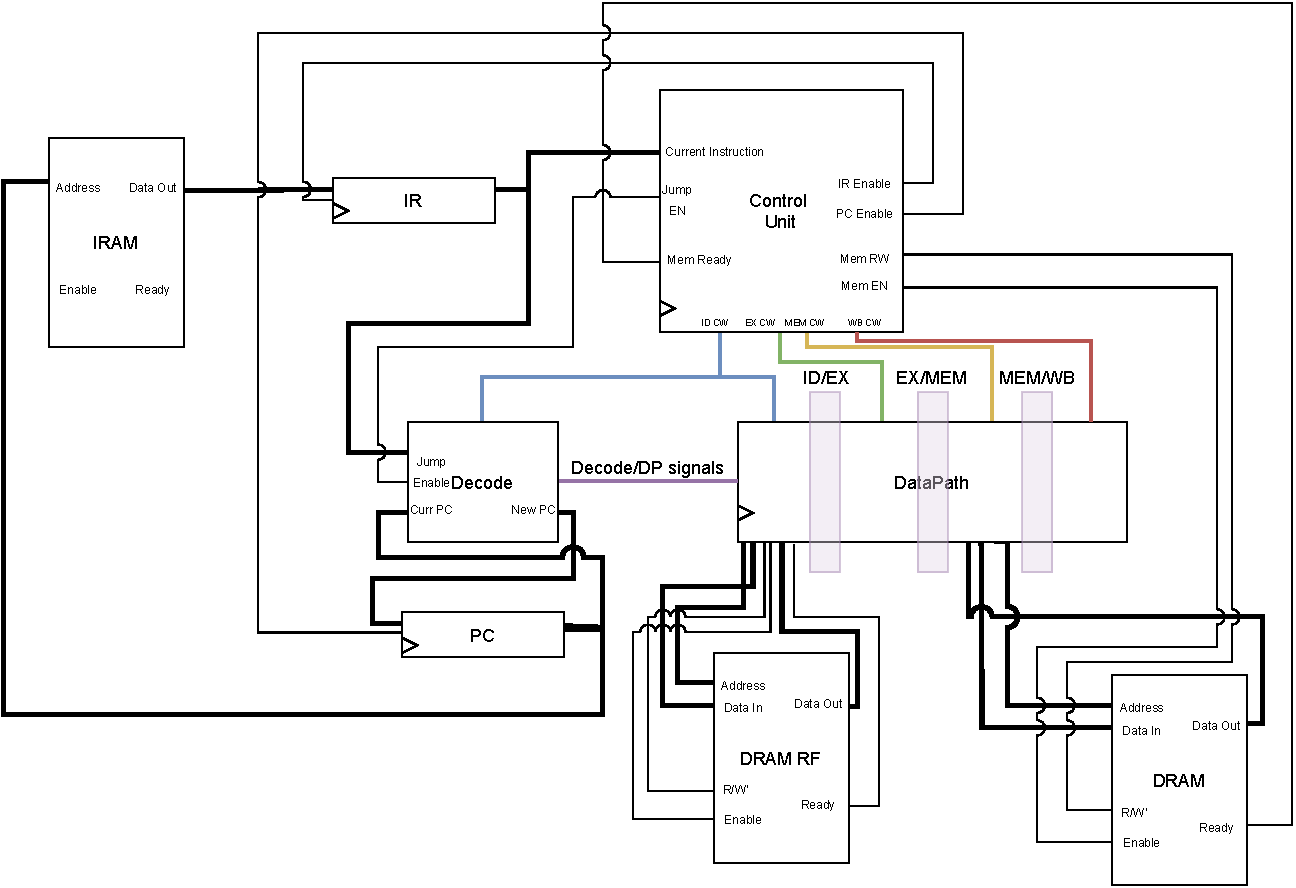
\includegraphics[width=1\textwidth]{chapters/2_dlx/images/DLX.pdf}
    \caption{Schematic of the DLX}
    \label{DLX}
\end{figure} 

\newpage
\section{Pipeline Stages}

To exploit the performance of the DLX processor, a five pipeline stage is implemented. This is done to reduce the overall delay, and different instructions can be processed in various stages simultaneously.

\begin{figure}[H]
    \centering
    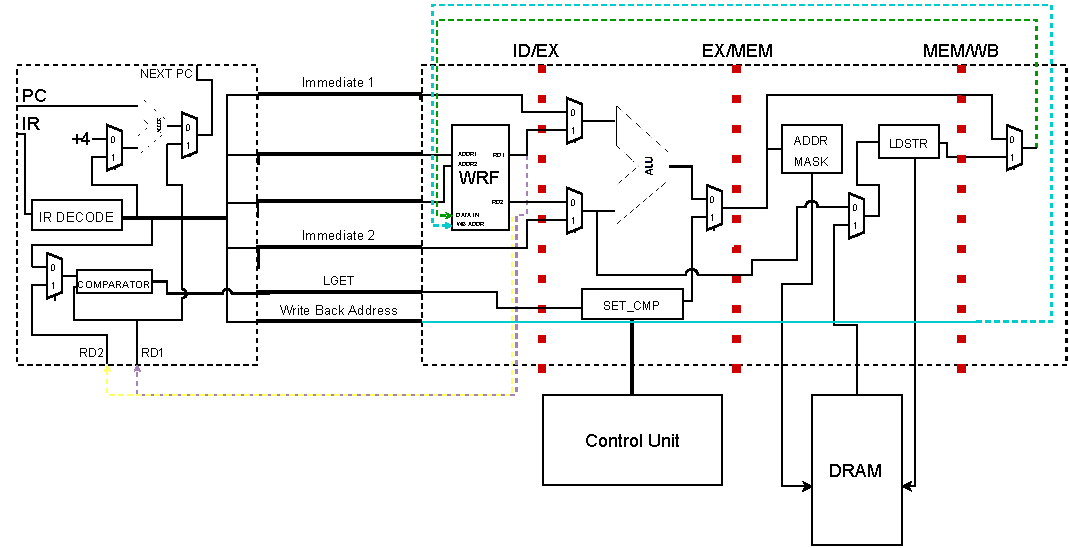
\includegraphics[width=0.91\textwidth]{chapters/2_dlx/images/DLX_DP.pdf}
    \caption{Schematic of the DLX Pipeline Structure}
    \label{DLX_DP}
\end{figure} 

As shown in figure \ref{DLX_DP}, the five pipeline stages are:

\begin{enumerate}
    \item \emph{Fetch}: not shown in the figure, it keeps track of the current instruction (IR) and the address of the next instruction to be fetched (PC).
    \item \emph{Decode}: it has the role of taking as input the current instruction (IR) and decoding it by extracting all the fields and dispatch them to the correct ports (Immediate 1, RS1, RS2, WB ADDR, Immediate 2). Furthermore, it's in charge of comparing values (from the Register File or an immediate) and computing the next PC given the actual PC. Last but not least, it keeps track of all the instructions in execution inside the pipeline and signals possible Data Hazard to the Control unit. By design choice, the Branch/Jump instructions are executed here instead of the Execute Stage, to lose only one clock cycle after a taken jump ideally (because of the wrong fetched instruction).
    \item \emph{Execute}: it takes the data from the Decode stage. Then, it does some computation on them, like adding them, multiply them, compute a shift and so on (refer to Table \ref{tab:alu_op} for available ALU operations), or outputs to the next stage the result of the comparison made in the Decode stage.
    \item \emph{Memory}: given the Address computed by the ALU during the previous stage and an optional Data, it's capable of doing a Load from the DRAM or a Store towards the DRAM. However, not all operations use this stage, so there is a bypass connection from the output of the EX stage towards the WB stage.
    \item \emph{Write Back}: the last stage of the pipeline selects the output from the ALU or the Memory (after a load operation) and gives it input to the Register File. Meanwhile, the destination address has been propagated through each stage and is now ready to be used by the Register File to store the final result. The Hazard Control Unit inside the Decode Stage intercepts this Write Back operation and knows that new instructions requiring this Data can now be executed.
\end{enumerate}


\section{Control Unit}

The Control Unit is one of the essential parts of the DLX processor. Its role is to orchestrate all the jobs through the processor's pipeline and manage dangerous situations.\\

Its interface is made of input signals (status signals from other components) and of control signals (towards other components), as described in Table \ref{table:cu:input_signals} and Table \ref{table:cu:output_signals}.

\begin{table}[H]
    \centering
    \begin{tabular}{l|l}
        \textbf{Signal Name} & \textbf{Description}\\
        \hline
        IR\_IN & Fetched Instruction, output from the IR Register \\
        HAZARD\_SIG & The Decode Stage is signaling a Hazard situation \\
        BUSY\_WINDOW & The Current RF Window has some registers in use \\
        SPILL & The Register File has started a push operations towards the memory \\
        FILL & The Register File has started a pop operations from the memory \\
        IRAM\_READY & The Instruction Memory has a data ready as output \\
        LGET & Comparison status from the comparator inside the Decode Unit\\
        DRAM\_READY & Indicates if the DRAM is ready or not\\
    \end{tabular}
    \caption{Input signals towards the Control Unit}
    \label{table:cu:input_signals}
\end{table}

\begin{table}[H]
    \centering
    \begin{tabular}{l|c|l}
        \textbf{Signal Name} & Sign & \textbf{Description}\\
        \hline
        PIPLIN\_IF\_EN & F & IF Stage enable: enable of IR register \\
        IF\_STALL & S & IF Stage stall: a NOP is insterted in the IR register \\
        PC\_EN & P & Enable of the PC register \\
        JUMP\_EN & J & JUMP must occur: Decode Stage will compute the new PC \\
        CALL & L & The Register File starts the context switch in a new window\\
        RET & E & The Register File must restore the previous window\\
        SEL\_CMPB & P & Reg or Imm field as comparator input in the Decode Stage\\
        UNSIGNED\_ID & U & All arithmetic units must consider operands as unsigned\\
        NPC\_SEL & N & Selects new PC (Adder or REG content)\\
        HAZARD\_TABLE\_WR1 & H & Enables log of the current instruction in the hazard control\\
        RF\_RD1\_EN & 1 & Enables the Read Port 1 in the RF\\
        RF\_RD2\_EN & 2 & Enables the Read Port 2 in the RF\\
        PIPLIN\_ID\_EN & D & ID Stage enable: enables all the ID pipeline REGs\\
        PIPLIN\_EX\_EN & X & EX Stage enable: enables all the EX pipeline REGs\\
        MUXA\_SEL & A & Input A of ALU: Immediate 1 or RD1\\
        MUXB\_SEL & B & Input B of ALU: Immediate 2 or RD2\\
        SEL\_ALU\_SETCMP & T & ALU or SET Comparator as EX stage output\\
        ALU\_OPCODE & \texttt{ALU} & ALU operation to be done\\
        SEL\_LGET & \texttt{SEL} & SET Comparator operation to be done\\
        DRAM\_WE & W & Enables the Write Operation in the DRAM\\
        DRAM\_RE & R & Enables the Read Operation in the DRAM\\
        DRAM\_ME & & Enable signal for the DRAM\\
        DATA\_SIZE & DS & Indicates the data of transfer towards/from the DRAM\\
        UNSIG\_SIGN\_N & U & Same as \emph{UNSIGNED\_ID} but 2 clock cycles delayed\\
        PIPLIN\_MEM\_EN & M & MEM Stage enable: enables all the MEM pipeline REGs\\
        WB\_MUX\_SEL & C & Selects MEM output or ALU out as content to write back\\
        PIPLIN\_WB\_EN & K & WB Stage enable: enables the Write signal in the RF\\
    \end{tabular}
    \caption{Output signals towards the Control Unit}
    \label{table:cu:output_signals}
\end{table}


\subsection{Control Words}

Going deeper into the Control Unit, we can look at the generated Control Words for each Instruction. Each bit is referred to a Control Signal as indicated in Table \ref{table:cu:output_signals}, \emph{Sign} column, while a blank bit means that it's randomly assigned.

\begin{figure}[ht]
    \begin{center}
        \begin{bytefield}[endianness=big,bitwidth=0.03\linewidth]{32}
        \bitheader{0-31} \\
            \bitbox{1}{F} & \bitbox{1}{S} & \bitbox{1}{P} & \bitbox{1}{J} & \bitbox{1}{L} & \bitbox{1}{E} & \bitbox{1}{1} & \bitbox{1}{2} & \bitbox{1}{P} & \bitbox{1}{U} & \bitbox{1}{N} & \bitbox{1}{H} & \bitbox{1}{D} & \bitbox{1}{X} & \bitbox{1}{A} & \bitbox{1}{B} & \bitbox{5}{ALU} & \bitbox{3}{SEL} & \bitbox{1}{T} & \bitbox{1}{W} & \bitbox{1}{R} & \bitbox{2}{DS} & \bitbox{1}{M} & \bitbox{1}{C} & \bitbox{1}{K}
        \end{bytefield}
    \end{center}
    \caption{Control Word bits organization}
\end{figure}


\begin{figure}[H]
    \begin{center}
        \begin{bytefield}[endianness=big,bitwidth=0.0278\linewidth]{32}
        \bitheader{0-10, 11, 15, 16-31} \\

        \begin{rightwordgroup}{RTYPE}
            \bitbox{1}{1} & \bitbox{1}{0} & \bitbox{1}{1} & \bitbox{1}{0} & \bitbox{1}{0} & \bitbox{1}{0} & \bitbox{1}{1} & \bitbox{1}{1} & \bitbox{1}{1} & \bitbox{1}{0} & \bitbox{1}{0} & \bitbox{1}{1} & \bitbox{1}{1} & \bitbox{1}{1} & \bitbox{1}{0} & \bitbox{1}{0} & \bitbox{5}{} & \bitbox{3}{} & \bitbox{1}{0} & \bitbox{1}{0} & \bitbox{1}{0} & \bitbox{2}{00} & \bitbox{1}{1} & \bitbox{1}{0} & \bitbox{1}{1}
        \end{rightwordgroup}\\

        \begin{rightwordgroup}{J}
            \bitbox{1}{1} & \bitbox{1}{1} & \bitbox{1}{1} & \bitbox{1}{1} & \bitbox{1}{0} & \bitbox{1}{0} & \bitbox{1}{0} & \bitbox{1}{0} & \bitbox{1}{1} & \bitbox{1}{0} & \bitbox{1}{0} & \bitbox{1}{0} & \bitbox{1}{0} & \bitbox{1}{0} & \bitbox{1}{0} & \bitbox{1}{0} & \bitbox{5}{ADD} & \bitbox{3}{SEQ} & \bitbox{1}{0} & \bitbox{1}{0} & \bitbox{1}{0} & \bitbox{2}{00} & \bitbox{1}{0} & \bitbox{1}{0} & \bitbox{1}{0}
        \end{rightwordgroup}\\

        \begin{rightwordgroup}{JAL}
            \bitbox{1}{1} & \bitbox{1}{1} & \bitbox{1}{1} & \bitbox{1}{1} & \bitbox{1}{0} & \bitbox{1}{0} & \bitbox{1}{1} & \bitbox{1}{0} & \bitbox{1}{1} & \bitbox{1}{0} & \bitbox{1}{0} & \bitbox{1}{1} & \bitbox{1}{1} & \bitbox{1}{1} & \bitbox{1}{0} & \bitbox{1}{1} & \bitbox{5}{ADD} & \bitbox{3}{SEQ} & \bitbox{1}{0} & \bitbox{1}{0} & \bitbox{1}{0} & \bitbox{2}{00} & \bitbox{1}{1} & \bitbox{1}{0} & \bitbox{1}{1}
        \end{rightwordgroup}\\


        \end{bytefield}
    \end{center}
    \caption{Control Word for each instruction}
\end{figure}


\begin{figure}[H]
    \begin{center}
        \begin{bytefield}[endianness=big,bitwidth=0.0278\linewidth]{32}
        \bitheader{0-10, 11, 15, 16-31} \\

        \begin{rightwordgroup}{BEQZ}
            \bitbox{1}{1} & \bitbox{1}{0} & \bitbox{1}{1} & \bitbox{1}{ } & \bitbox{1}{0} & \bitbox{1}{0} & \bitbox{1}{1} & \bitbox{1}{1} & \bitbox{1}{1} & \bitbox{1}{0} & \bitbox{1}{0} & \bitbox{1}{0} & \bitbox{1}{0} & \bitbox{1}{0} & \bitbox{1}{0} & \bitbox{1}{0} & \bitbox{5}{ADD} & \bitbox{3}{SEQ} & \bitbox{1}{0} & \bitbox{1}{0} & \bitbox{1}{0} & \bitbox{2}{00} & \bitbox{1}{0} & \bitbox{1}{0} & \bitbox{1}{0}
        \end{rightwordgroup}\\

        \begin{rightwordgroup}{BNEZ}
            \bitbox{1}{1} & \bitbox{1}{0} & \bitbox{1}{1} & \bitbox{1}{ } & \bitbox{1}{0} & \bitbox{1}{0} & \bitbox{1}{1} & \bitbox{1}{1} & \bitbox{1}{1} & \bitbox{1}{0} & \bitbox{1}{0} & \bitbox{1}{0} & \bitbox{1}{0} & \bitbox{1}{0} & \bitbox{1}{0} & \bitbox{1}{0} & \bitbox{5}{ADD} & \bitbox{3}{SEQ} & \bitbox{1}{0} & \bitbox{1}{0} & \bitbox{1}{0} & \bitbox{2}{00} & \bitbox{1}{0} & \bitbox{1}{0} & \bitbox{1}{0}
        \end{rightwordgroup}\\

        \begin{rightwordgroup}{ADDI}
            \bitbox{1}{1} & \bitbox{1}{0} & \bitbox{1}{1} & \bitbox{1}{0} & \bitbox{1}{0} & \bitbox{1}{0} & \bitbox{1}{1} & \bitbox{1}{0} & \bitbox{1}{0} & \bitbox{1}{0} & \bitbox{1}{0} & \bitbox{1}{1} & \bitbox{1}{1} & \bitbox{1}{1} & \bitbox{1}{0} & \bitbox{1}{1} & \bitbox{5}{ADD} & \bitbox{3}{SEQ} & \bitbox{1}{0} & \bitbox{1}{0} & \bitbox{1}{0} & \bitbox{2}{00} & \bitbox{1}{1} & \bitbox{1}{0} & \bitbox{1}{1}
        \end{rightwordgroup}\\

        \begin{rightwordgroup}{ADDUI}
            \bitbox{1}{1} & \bitbox{1}{0} & \bitbox{1}{1} & \bitbox{1}{0} & \bitbox{1}{0} & \bitbox{1}{0} & \bitbox{1}{1} & \bitbox{1}{0} & \bitbox{1}{0} & \bitbox{1}{1} & \bitbox{1}{0} & \bitbox{1}{1} & \bitbox{1}{1} & \bitbox{1}{1} & \bitbox{1}{0} & \bitbox{1}{1} & \bitbox{5}{ADD} & \bitbox{3}{SEQ} & \bitbox{1}{0} & \bitbox{1}{0} & \bitbox{1}{0} & \bitbox{2}{00} & \bitbox{1}{1} & \bitbox{1}{0} & \bitbox{1}{1}
        \end{rightwordgroup}\\

        \begin{rightwordgroup}{SUBI}
            \bitbox{1}{1} & \bitbox{1}{0} & \bitbox{1}{1} & \bitbox{1}{0} & \bitbox{1}{0} & \bitbox{1}{0} & \bitbox{1}{1} & \bitbox{1}{0} & \bitbox{1}{0} & \bitbox{1}{0} & \bitbox{1}{0} & \bitbox{1}{1} & \bitbox{1}{1} & \bitbox{1}{1} & \bitbox{1}{0} & \bitbox{1}{1} & \bitbox{5}{SUB} & \bitbox{3}{SEQ} & \bitbox{1}{0} & \bitbox{1}{0} & \bitbox{1}{0} & \bitbox{2}{00} & \bitbox{1}{1} & \bitbox{1}{0} & \bitbox{1}{1}
        \end{rightwordgroup}\\

        \begin{rightwordgroup}{SUBUI}
            \bitbox{1}{1} & \bitbox{1}{0} & \bitbox{1}{1} & \bitbox{1}{0} & \bitbox{1}{0} & \bitbox{1}{0} & \bitbox{1}{1} & \bitbox{1}{0} & \bitbox{1}{0} & \bitbox{1}{1} & \bitbox{1}{0} & \bitbox{1}{1} & \bitbox{1}{1} & \bitbox{1}{1} & \bitbox{1}{0} & \bitbox{1}{1} & \bitbox{5}{SUB} & \bitbox{3}{SEQ} & \bitbox{1}{0} & \bitbox{1}{0} & \bitbox{1}{0} & \bitbox{2}{00} & \bitbox{1}{1} & \bitbox{1}{0} & \bitbox{1}{1}
        \end{rightwordgroup}\\

        \begin{rightwordgroup}{ANDI}
            \bitbox{1}{1} & \bitbox{1}{0} & \bitbox{1}{1} & \bitbox{1}{0} & \bitbox{1}{0} & \bitbox{1}{0} & \bitbox{1}{1} & \bitbox{1}{0} & \bitbox{1}{0} & \bitbox{1}{1} & \bitbox{1}{0} & \bitbox{1}{1} & \bitbox{1}{1} & \bitbox{1}{1} & \bitbox{1}{0} & \bitbox{1}{1} & \bitbox{5}{AND} & \bitbox{3}{SEQ} & \bitbox{1}{0} & \bitbox{1}{0} & \bitbox{1}{0} & \bitbox{2}{00} & \bitbox{1}{1} & \bitbox{1}{0} & \bitbox{1}{1}
        \end{rightwordgroup}\\

        \begin{rightwordgroup}{ORI}
            \bitbox{1}{1} & \bitbox{1}{0} & \bitbox{1}{1} & \bitbox{1}{0} & \bitbox{1}{0} & \bitbox{1}{0} & \bitbox{1}{1} & \bitbox{1}{0} & \bitbox{1}{0} & \bitbox{1}{1} & \bitbox{1}{0} & \bitbox{1}{1} & \bitbox{1}{1} & \bitbox{1}{1} & \bitbox{1}{0} & \bitbox{1}{1} & \bitbox{5}{OR} & \bitbox{3}{SEQ} & \bitbox{1}{0} & \bitbox{1}{0} & \bitbox{1}{0} & \bitbox{2}{00} & \bitbox{1}{1} & \bitbox{1}{0} & \bitbox{1}{1}
        \end{rightwordgroup}\\

        \begin{rightwordgroup}{XORI}
            \bitbox{1}{1} & \bitbox{1}{0} & \bitbox{1}{1} & \bitbox{1}{0} & \bitbox{1}{0} & \bitbox{1}{0} & \bitbox{1}{1} & \bitbox{1}{0} & \bitbox{1}{0} & \bitbox{1}{1} & \bitbox{1}{0} & \bitbox{1}{1} & \bitbox{1}{1} & \bitbox{1}{1} & \bitbox{1}{0} & \bitbox{1}{1} & \bitbox{5}{XOR} & \bitbox{3}{SEQ} & \bitbox{1}{0} & \bitbox{1}{0} & \bitbox{1}{0} & \bitbox{2}{00} & \bitbox{1}{1} & \bitbox{1}{0} & \bitbox{1}{1}
        \end{rightwordgroup}\\

        \begin{rightwordgroup}{LHI}
            \bitbox{1}{1} & \bitbox{1}{0} & \bitbox{1}{1} & \bitbox{1}{0} & \bitbox{1}{0} & \bitbox{1}{0} & \bitbox{1}{0} & \bitbox{1}{0} & \bitbox{1}{0} & \bitbox{1}{0} & \bitbox{1}{0} & \bitbox{1}{1} & \bitbox{1}{1} & \bitbox{1}{1} & \bitbox{1}{1} & \bitbox{1}{1} & \bitbox{5}{SLL} & \bitbox{3}{SEQ} & \bitbox{1}{0} & \bitbox{1}{0} & \bitbox{1}{0} & \bitbox{2}{00} & \bitbox{1}{1} & \bitbox{1}{0} & \bitbox{1}{1}
        \end{rightwordgroup}\\

        \begin{rightwordgroup}{JR}
            \bitbox{1}{1} & \bitbox{1}{1} & \bitbox{1}{1} & \bitbox{1}{1} & \bitbox{1}{0} & \bitbox{1}{0} & \bitbox{1}{1} & \bitbox{1}{0} & \bitbox{1}{1} & \bitbox{1}{0} & \bitbox{1}{1} & \bitbox{1}{0} & \bitbox{1}{0} & \bitbox{1}{0} & \bitbox{1}{0} & \bitbox{1}{0} & \bitbox{5}{ADD} & \bitbox{3}{SEQ} & \bitbox{1}{0} & \bitbox{1}{0} & \bitbox{1}{0} & \bitbox{2}{00} & \bitbox{1}{0} & \bitbox{1}{0} & \bitbox{1}{0}
        \end{rightwordgroup}\\

        \begin{rightwordgroup}{JALR}
            \bitbox{1}{1} & \bitbox{1}{1} & \bitbox{1}{1} & \bitbox{1}{1} & \bitbox{1}{0} & \bitbox{1}{0} & \bitbox{1}{1} & \bitbox{1}{1} & \bitbox{1}{1} & \bitbox{1}{0} & \bitbox{1}{1} & \bitbox{1}{1} & \bitbox{1}{1} & \bitbox{1}{1} & \bitbox{1}{0} & \bitbox{1}{1} & \bitbox{5}{ADD} & \bitbox{3}{SEQ} & \bitbox{1}{0} & \bitbox{1}{0} & \bitbox{1}{0} & \bitbox{2}{00} & \bitbox{1}{1} & \bitbox{1}{0} & \bitbox{1}{1}
        \end{rightwordgroup}\\

        \begin{rightwordgroup}{SLLI}
            \bitbox{1}{1} & \bitbox{1}{0} & \bitbox{1}{1} & \bitbox{1}{0} & \bitbox{1}{0} & \bitbox{1}{0} & \bitbox{1}{1} & \bitbox{1}{0} & \bitbox{1}{0} & \bitbox{1}{1} & \bitbox{1}{0} & \bitbox{1}{1} & \bitbox{1}{1} & \bitbox{1}{1} & \bitbox{1}{0} & \bitbox{1}{1} & \bitbox{5}{SLL} & \bitbox{3}{SEQ} & \bitbox{1}{0} & \bitbox{1}{0} & \bitbox{1}{0} & \bitbox{2}{00} & \bitbox{1}{1} & \bitbox{1}{0} & \bitbox{1}{1}
        \end{rightwordgroup}\\

        \begin{rightwordgroup}{NOP}
            \bitbox{1}{1} & \bitbox{1}{0} & \bitbox{1}{1} & \bitbox{1}{0} & \bitbox{1}{0} & \bitbox{1}{0} & \bitbox{1}{0} & \bitbox{1}{0} & \bitbox{1}{1} & \bitbox{1}{0} & \bitbox{1}{0} & \bitbox{1}{0} & \bitbox{1}{0} & \bitbox{1}{0} & \bitbox{1}{0} & \bitbox{1}{0} & \bitbox{5}{ADD} & \bitbox{3}{SEQ} & \bitbox{1}{0} & \bitbox{1}{0} & \bitbox{1}{0} & \bitbox{2}{00} & \bitbox{1}{0} & \bitbox{1}{0} & \bitbox{1}{0}
        \end{rightwordgroup}\\

        \begin{rightwordgroup}{SRLI}
            \bitbox{1}{1} & \bitbox{1}{0} & \bitbox{1}{1} & \bitbox{1}{0} & \bitbox{1}{0} & \bitbox{1}{0} & \bitbox{1}{1} & \bitbox{1}{0} & \bitbox{1}{0} & \bitbox{1}{1} & \bitbox{1}{0} & \bitbox{1}{1} & \bitbox{1}{1} & \bitbox{1}{1} & \bitbox{1}{0} & \bitbox{1}{1} & \bitbox{5}{SRL} & \bitbox{3}{SEQ} & \bitbox{1}{0} & \bitbox{1}{0} & \bitbox{1}{0} & \bitbox{2}{00} & \bitbox{1}{1} & \bitbox{1}{0} & \bitbox{1}{1}
        \end{rightwordgroup}\\

        \begin{rightwordgroup}{SRAI}
            \bitbox{1}{1} & \bitbox{1}{0} & \bitbox{1}{1} & \bitbox{1}{0} & \bitbox{1}{0} & \bitbox{1}{0} & \bitbox{1}{1} & \bitbox{1}{0} & \bitbox{1}{1} & \bitbox{1}{1} & \bitbox{1}{0} & \bitbox{1}{1} & \bitbox{1}{1} & \bitbox{1}{1} & \bitbox{1}{0} & \bitbox{1}{1} & \bitbox{5}{SRA} & \bitbox{3}{SEQ} & \bitbox{1}{0} & \bitbox{1}{0} & \bitbox{1}{0} & \bitbox{2}{00} & \bitbox{1}{1} & \bitbox{1}{0} & \bitbox{1}{1}
        \end{rightwordgroup}\\

        \begin{rightwordgroup}{SEQI}
            \bitbox{1}{1} & \bitbox{1}{0} & \bitbox{1}{1} & \bitbox{1}{0} & \bitbox{1}{0} & \bitbox{1}{0} & \bitbox{1}{1} & \bitbox{1}{0} & \bitbox{1}{0} & \bitbox{1}{0} & \bitbox{1}{0} & \bitbox{1}{1} & \bitbox{1}{1} & \bitbox{1}{1} & \bitbox{1}{0} & \bitbox{1}{1} & \bitbox{5}{ADD} & \bitbox{3}{SEQ} & \bitbox{1}{1} & \bitbox{1}{0} & \bitbox{1}{0} & \bitbox{2}{00} & \bitbox{1}{1} & \bitbox{1}{0} & \bitbox{1}{1}
        \end{rightwordgroup}\\

        \begin{rightwordgroup}{SNEI}
            \bitbox{1}{1} & \bitbox{1}{0} & \bitbox{1}{1} & \bitbox{1}{0} & \bitbox{1}{0} & \bitbox{1}{0} & \bitbox{1}{1} & \bitbox{1}{0} & \bitbox{1}{0} & \bitbox{1}{0} & \bitbox{1}{0} & \bitbox{1}{1} & \bitbox{1}{1} & \bitbox{1}{1} & \bitbox{1}{0} & \bitbox{1}{1} & \bitbox{5}{ADD} & \bitbox{3}{SNE} & \bitbox{1}{1} & \bitbox{1}{0} & \bitbox{1}{0} & \bitbox{2}{00} & \bitbox{1}{1} & \bitbox{1}{0} & \bitbox{1}{1}
        \end{rightwordgroup}\\

        \begin{rightwordgroup}{SLTI}
            \bitbox{1}{1} & \bitbox{1}{0} & \bitbox{1}{1} & \bitbox{1}{0} & \bitbox{1}{0} & \bitbox{1}{0} & \bitbox{1}{1} & \bitbox{1}{0} & \bitbox{1}{0} & \bitbox{1}{0} & \bitbox{1}{0} & \bitbox{1}{1} & \bitbox{1}{1} & \bitbox{1}{1} & \bitbox{1}{0} & \bitbox{1}{1} & \bitbox{5}{ADD} & \bitbox{3}{SLT} & \bitbox{1}{1} & \bitbox{1}{0} & \bitbox{1}{0} & \bitbox{2}{00} & \bitbox{1}{1} & \bitbox{1}{0} & \bitbox{1}{1}
        \end{rightwordgroup}\\

        \begin{rightwordgroup}{SGTI}
                \bitbox{1}{1} & \bitbox{1}{0} & \bitbox{1}{1} & \bitbox{1}{0} & \bitbox{1}{0} & \bitbox{1}{0} & \bitbox{1}{1} & \bitbox{1}{0} & \bitbox{1}{0} & \bitbox{1}{0} & \bitbox{1}{0} & \bitbox{1}{1} & \bitbox{1}{1} & \bitbox{1}{1} & \bitbox{1}{0} & \bitbox{1}{1} & \bitbox{5}{ADD} & \bitbox{3}{SGT} & \bitbox{1}{1} & \bitbox{1}{0} & \bitbox{1}{0} & \bitbox{2}{00} & \bitbox{1}{1} & \bitbox{1}{0} & \bitbox{1}{1}
        \end{rightwordgroup}\\

        \begin{rightwordgroup}{SLEI}
            \bitbox{1}{1} & \bitbox{1}{0} & \bitbox{1}{1} & \bitbox{1}{0} & \bitbox{1}{0} & \bitbox{1}{0} & \bitbox{1}{1} & \bitbox{1}{0} & \bitbox{1}{0} & \bitbox{1}{0} & \bitbox{1}{0} & \bitbox{1}{1} & \bitbox{1}{1} & \bitbox{1}{1} & \bitbox{1}{0} & \bitbox{1}{1} & \bitbox{5}{ADD} & \bitbox{3}{SLE} & \bitbox{1}{1} & \bitbox{1}{0} & \bitbox{1}{0} & \bitbox{2}{00} & \bitbox{1}{1} & \bitbox{1}{0} & \bitbox{1}{1}
        \end{rightwordgroup}\\

        \begin{rightwordgroup}{SGEI}
            \bitbox{1}{1} & \bitbox{1}{0} & \bitbox{1}{1} & \bitbox{1}{0} & \bitbox{1}{0} & \bitbox{1}{0} & \bitbox{1}{1} & \bitbox{1}{0} & \bitbox{1}{0} & \bitbox{1}{0} & \bitbox{1}{0} & \bitbox{1}{1} & \bitbox{1}{1} & \bitbox{1}{1} & \bitbox{1}{0} & \bitbox{1}{1} & \bitbox{5}{ADD} & \bitbox{3}{SGE} & \bitbox{1}{1} & \bitbox{1}{0} & \bitbox{1}{0} & \bitbox{2}{00} & \bitbox{1}{1} & \bitbox{1}{0} & \bitbox{1}{1}
        \end{rightwordgroup}\\

        \begin{rightwordgroup}{CALL}
            \bitbox{1}{1} & \bitbox{1}{1} & \bitbox{1}{1} & \bitbox{1}{1} & \bitbox{1}{0} & \bitbox{1}{0} & \bitbox{1}{1} & \bitbox{1}{0} & \bitbox{1}{1} & \bitbox{1}{0} & \bitbox{1}{0} & \bitbox{1}{1} & \bitbox{1}{1} & \bitbox{1}{1} & \bitbox{1}{0} & \bitbox{1}{1} & \bitbox{5}{ADD} & \bitbox{3}{SEQ} & \bitbox{1}{0} & \bitbox{1}{0} & \bitbox{1}{0} & \bitbox{2}{00} & \bitbox{1}{1} & \bitbox{1}{0} & \bitbox{1}{1}
        \end{rightwordgroup}\\

        \begin{rightwordgroup}{RET}
            \bitbox{1}{1} & \bitbox{1}{1} & \bitbox{1}{1} & \bitbox{1}{1} & \bitbox{1}{0} & \bitbox{1}{1} & \bitbox{1}{1} & \bitbox{1}{0} & \bitbox{1}{0} & \bitbox{1}{0} & \bitbox{1}{1} & \bitbox{1}{0} & \bitbox{1}{0} & \bitbox{1}{0} & \bitbox{1}{0} & \bitbox{1}{0} & \bitbox{5}{ADD} & \bitbox{3}{SEQ} & \bitbox{1}{0} & \bitbox{1}{0} & \bitbox{1}{0} & \bitbox{2}{00} & \bitbox{1}{0} & \bitbox{1}{0} & \bitbox{1}{0}
        \end{rightwordgroup}\\

        \begin{rightwordgroup}{LB}
            \bitbox{1}{1} & \bitbox{1}{0} & \bitbox{1}{1} & \bitbox{1}{0} & \bitbox{1}{0} & \bitbox{1}{0} & \bitbox{1}{1} & \bitbox{1}{0} & \bitbox{1}{0} & \bitbox{1}{0} & \bitbox{1}{0} & \bitbox{1}{1} & \bitbox{1}{1} & \bitbox{1}{1} & \bitbox{1}{0} & \bitbox{1}{1} & \bitbox{5}{ADD} & \bitbox{3}{SEQ} & \bitbox{1}{0} & \bitbox{1}{0} & \bitbox{1}{1} & \bitbox{2}{10} & \bitbox{1}{1} & \bitbox{1}{1} & \bitbox{1}{1}
        \end{rightwordgroup}\\

        \begin{rightwordgroup}{LH}
            \bitbox{1}{1} & \bitbox{1}{0} & \bitbox{1}{1} & \bitbox{1}{0} & \bitbox{1}{0} & \bitbox{1}{0} & \bitbox{1}{1} & \bitbox{1}{0} & \bitbox{1}{0} & \bitbox{1}{0} & \bitbox{1}{0} & \bitbox{1}{1} & \bitbox{1}{1} & \bitbox{1}{1} & \bitbox{1}{0} & \bitbox{1}{1} & \bitbox{5}{ADD} & \bitbox{3}{SEQ} & \bitbox{1}{0} & \bitbox{1}{0} & \bitbox{1}{1} & \bitbox{2}{01} & \bitbox{1}{1} & \bitbox{1}{1} & \bitbox{1}{1}
        \end{rightwordgroup}\\

        \begin{rightwordgroup}{LW}
            \bitbox{1}{1} & \bitbox{1}{0} & \bitbox{1}{1} & \bitbox{1}{0} & \bitbox{1}{0} & \bitbox{1}{0} & \bitbox{1}{1} & \bitbox{1}{0} & \bitbox{1}{0} & \bitbox{1}{0} & \bitbox{1}{0} & \bitbox{1}{1} & \bitbox{1}{1} & \bitbox{1}{1} & \bitbox{1}{0} & \bitbox{1}{1} & \bitbox{5}{ADD} & \bitbox{3}{SEQ} & \bitbox{1}{0} & \bitbox{1}{0} & \bitbox{1}{1} & \bitbox{2}{00} & \bitbox{1}{1} & \bitbox{1}{1} & \bitbox{1}{1}
        \end{rightwordgroup}\\

        \begin{rightwordgroup}{LBU}
            \bitbox{1}{1} & \bitbox{1}{0} & \bitbox{1}{1} & \bitbox{1}{0} & \bitbox{1}{0} & \bitbox{1}{0} & \bitbox{1}{1} & \bitbox{1}{0} & \bitbox{1}{0} & \bitbox{1}{1} & \bitbox{1}{0} & \bitbox{1}{1} & \bitbox{1}{1} & \bitbox{1}{1} & \bitbox{1}{0} & \bitbox{1}{1} & \bitbox{5}{ADD} & \bitbox{3}{SEQ} & \bitbox{1}{0} & \bitbox{1}{0} & \bitbox{1}{1} & \bitbox{2}{10} & \bitbox{1}{1} & \bitbox{1}{1} & \bitbox{1}{1}
        \end{rightwordgroup}\\

        \begin{rightwordgroup}{LHU}
            \bitbox{1}{1} & \bitbox{1}{0} & \bitbox{1}{1} & \bitbox{1}{0} & \bitbox{1}{0} & \bitbox{1}{0} & \bitbox{1}{1} & \bitbox{1}{0} & \bitbox{1}{0} & \bitbox{1}{1} & \bitbox{1}{0} & \bitbox{1}{1} & \bitbox{1}{1} & \bitbox{1}{1} & \bitbox{1}{0} & \bitbox{1}{1} & \bitbox{5}{ADD} & \bitbox{3}{SEQ} & \bitbox{1}{0} & \bitbox{1}{0} & \bitbox{1}{1} & \bitbox{2}{01} & \bitbox{1}{1} & \bitbox{1}{1} & \bitbox{1}{1}
        \end{rightwordgroup}\\

        \begin{rightwordgroup}{SB}
            \bitbox{1}{1} & \bitbox{1}{0} & \bitbox{1}{1} & \bitbox{1}{0} & \bitbox{1}{0} & \bitbox{1}{0} & \bitbox{1}{1} & \bitbox{1}{1} & \bitbox{1}{0} & \bitbox{1}{0} & \bitbox{1}{0} & \bitbox{1}{0} & \bitbox{1}{1} & \bitbox{1}{1} & \bitbox{1}{0} & \bitbox{1}{1} & \bitbox{5}{ADD} & \bitbox{3}{SEQ} & \bitbox{1}{0} & \bitbox{1}{1} & \bitbox{1}{0} & \bitbox{2}{10} & \bitbox{1}{1} & \bitbox{1}{0} & \bitbox{1}{0}
        \end{rightwordgroup}\\

        \begin{rightwordgroup}{SH}
            \bitbox{1}{1} & \bitbox{1}{0} & \bitbox{1}{1} & \bitbox{1}{0} & \bitbox{1}{0} & \bitbox{1}{0} & \bitbox{1}{1} & \bitbox{1}{1} & \bitbox{1}{0} & \bitbox{1}{0} & \bitbox{1}{0} & \bitbox{1}{0} & \bitbox{1}{1} & \bitbox{1}{1} & \bitbox{1}{0} & \bitbox{1}{1} & \bitbox{5}{ADD} & \bitbox{3}{SEQ} & \bitbox{1}{0} & \bitbox{1}{1} & \bitbox{1}{0} & \bitbox{2}{01} & \bitbox{1}{1} & \bitbox{1}{0} & \bitbox{1}{0}
        \end{rightwordgroup}\\

        \begin{rightwordgroup}{SW}
            \bitbox{1}{1} & \bitbox{1}{0} & \bitbox{1}{1} & \bitbox{1}{0} & \bitbox{1}{0} & \bitbox{1}{0} & \bitbox{1}{1} & \bitbox{1}{1} & \bitbox{1}{0} & \bitbox{1}{0} & \bitbox{1}{0} & \bitbox{1}{0} & \bitbox{1}{1} & \bitbox{1}{1} & \bitbox{1}{0} & \bitbox{1}{1} & \bitbox{5}{ADD} & \bitbox{3}{SEQ} & \bitbox{1}{0} & \bitbox{1}{1} & \bitbox{1}{0} & \bitbox{2}{00} & \bitbox{1}{1} & \bitbox{1}{0} & \bitbox{1}{0}
        \end{rightwordgroup}\\


        \begin{rightwordgroup}{TKTM}
            \bitbox{1}{1} & \bitbox{1}{0} & \bitbox{1}{1} & \bitbox{1}{0} & \bitbox{1}{0} & \bitbox{1}{0} & \bitbox{1}{1} & \bitbox{1}{0} & \bitbox{1}{1} & \bitbox{1}{0} & \bitbox{1}{0} & \bitbox{1}{1} & \bitbox{1}{1} & \bitbox{1}{1} & \bitbox{1}{0} & \bitbox{1}{1} & \bitbox{5}{ADD} & \bitbox{3}{SEQ} & \bitbox{1}{0} & \bitbox{1}{0} & \bitbox{1}{0} & \bitbox{2}{00} & \bitbox{1}{1} & \bitbox{1}{0} & \bitbox{1}{1}
        \end{rightwordgroup}\\

        \begin{rightwordgroup}{SLTUI}
            \bitbox{1}{1} & \bitbox{1}{0} & \bitbox{1}{1} & \bitbox{1}{0} & \bitbox{1}{0} & \bitbox{1}{0} & \bitbox{1}{1} & \bitbox{1}{0} & \bitbox{1}{0} & \bitbox{1}{1} & \bitbox{1}{0} & \bitbox{1}{1} & \bitbox{1}{1} & \bitbox{1}{1} & \bitbox{1}{0} & \bitbox{1}{1} & \bitbox{5}{ADD} & \bitbox{3}{SLT} & \bitbox{1}{1} & \bitbox{1}{0} & \bitbox{1}{0} & \bitbox{2}{00} & \bitbox{1}{1} & \bitbox{1}{0} & \bitbox{1}{1}
        \end{rightwordgroup}\\

        \begin{rightwordgroup}{SGTUI}
            \bitbox{1}{1} & \bitbox{1}{0} & \bitbox{1}{1} & \bitbox{1}{0} & \bitbox{1}{0} & \bitbox{1}{0} & \bitbox{1}{1} & \bitbox{1}{0} & \bitbox{1}{0} & \bitbox{1}{1} & \bitbox{1}{0} & \bitbox{1}{1} & \bitbox{1}{1} & \bitbox{1}{1} & \bitbox{1}{0} & \bitbox{1}{1} & \bitbox{5}{ADD} & \bitbox{3}{SGT} & \bitbox{1}{1} & \bitbox{1}{0} & \bitbox{1}{0} & \bitbox{2}{00} & \bitbox{1}{1} & \bitbox{1}{0} & \bitbox{1}{1}
        \end{rightwordgroup}\\

        \begin{rightwordgroup}{SLEUI}
            \bitbox{1}{1} & \bitbox{1}{0} & \bitbox{1}{1} & \bitbox{1}{0} & \bitbox{1}{0} & \bitbox{1}{0} & \bitbox{1}{1} & \bitbox{1}{0} & \bitbox{1}{0} & \bitbox{1}{1} & \bitbox{1}{0} & \bitbox{1}{1} & \bitbox{1}{1} & \bitbox{1}{1} & \bitbox{1}{0} & \bitbox{1}{1} & \bitbox{5}{ADD} & \bitbox{3}{SLE} & \bitbox{1}{1} & \bitbox{1}{0} & \bitbox{1}{0} & \bitbox{2}{00} & \bitbox{1}{1} & \bitbox{1}{0} & \bitbox{1}{1}
        \end{rightwordgroup}\\

        \begin{rightwordgroup}{SGEUI}
            \bitbox{1}{1} & \bitbox{1}{0} & \bitbox{1}{1} & \bitbox{1}{0} & \bitbox{1}{0} & \bitbox{1}{0} & \bitbox{1}{1} & \bitbox{1}{0} & \bitbox{1}{0} & \bitbox{1}{1} & \bitbox{1}{0} & \bitbox{1}{1} & \bitbox{1}{1} & \bitbox{1}{1} & \bitbox{1}{0} & \bitbox{1}{1} & \bitbox{5}{ADD} & \bitbox{3}{SGE} & \bitbox{1}{1} & \bitbox{1}{0} & \bitbox{1}{0} & \bitbox{2}{00} & \bitbox{1}{1} & \bitbox{1}{0} & \bitbox{1}{1}
        \end{rightwordgroup}\\


        \begin{rightwordgroup}{BGT}
            \bitbox{1}{1} & \bitbox{1}{0} & \bitbox{1}{1} & \bitbox{1}{} & \bitbox{1}{0} & \bitbox{1}{0} & \bitbox{1}{1} & \bitbox{1}{1} & \bitbox{1}{1} & \bitbox{1}{0} & \bitbox{1}{0} & \bitbox{1}{0} & \bitbox{1}{0} & \bitbox{1}{0} & \bitbox{1}{0} & \bitbox{1}{0} & \bitbox{5}{ADD} & \bitbox{3}{SEQ} & \bitbox{1}{0} & \bitbox{1}{0} & \bitbox{1}{0} & \bitbox{2}{00} & \bitbox{1}{0} & \bitbox{1}{0} & \bitbox{1}{0}
        \end{rightwordgroup}\\

        \begin{rightwordgroup}{BGE}
            \bitbox{1}{1} & \bitbox{1}{0} & \bitbox{1}{1} & \bitbox{1}{} & \bitbox{1}{0} & \bitbox{1}{0} & \bitbox{1}{1} & \bitbox{1}{1} & \bitbox{1}{1} & \bitbox{1}{0} & \bitbox{1}{0} & \bitbox{1}{0} & \bitbox{1}{0} & \bitbox{1}{0} & \bitbox{1}{0} & \bitbox{1}{0} & \bitbox{5}{ADD} & \bitbox{3}{SEQ} & \bitbox{1}{0} & \bitbox{1}{0} & \bitbox{1}{0} & \bitbox{2}{00} & \bitbox{1}{0} & \bitbox{1}{0} & \bitbox{1}{0}
        \end{rightwordgroup}\\

        \begin{rightwordgroup}{BLT}
            \bitbox{1}{1} & \bitbox{1}{0} & \bitbox{1}{1} & \bitbox{1}{} & \bitbox{1}{0} & \bitbox{1}{0} & \bitbox{1}{1} & \bitbox{1}{1} & \bitbox{1}{1} & \bitbox{1}{0} & \bitbox{1}{0} & \bitbox{1}{0} & \bitbox{1}{0} & \bitbox{1}{0} & \bitbox{1}{0} & \bitbox{1}{0} & \bitbox{5}{ADD} & \bitbox{3}{SEQ} & \bitbox{1}{0} & \bitbox{1}{0} & \bitbox{1}{0} & \bitbox{2}{00} & \bitbox{1}{0} & \bitbox{1}{0} & \bitbox{1}{0}
        \end{rightwordgroup}\\

        \begin{rightwordgroup}{BLE}
            \bitbox{1}{1} & \bitbox{1}{0} & \bitbox{1}{1} & \bitbox{1}{} & \bitbox{1}{0} & \bitbox{1}{0} & \bitbox{1}{1} & \bitbox{1}{1} & \bitbox{1}{1} & \bitbox{1}{0} & \bitbox{1}{0} & \bitbox{1}{0} & \bitbox{1}{0} & \bitbox{1}{0} & \bitbox{1}{0} & \bitbox{1}{0} & \bitbox{5}{ADD} & \bitbox{3}{SEQ} & \bitbox{1}{0} & \bitbox{1}{0} & \bitbox{1}{0} & \bitbox{2}{00} & \bitbox{1}{0} & \bitbox{1}{0} & \bitbox{1}{0}
        \end{rightwordgroup}\\

        \end{bytefield}
    \end{center}
    \caption{Control Word for each instruction}
\end{figure}




\subsection{Internal organization of the Control Unit}

The Control Unit internally is organized mainly with a stage that converts the actual Instruction into a Control Word. Then this control word is propagated to support all the pipeline stages, as shown in Figure \ref{dlx:cu:schematic}.

\begin{figure}[H]
    \centering
    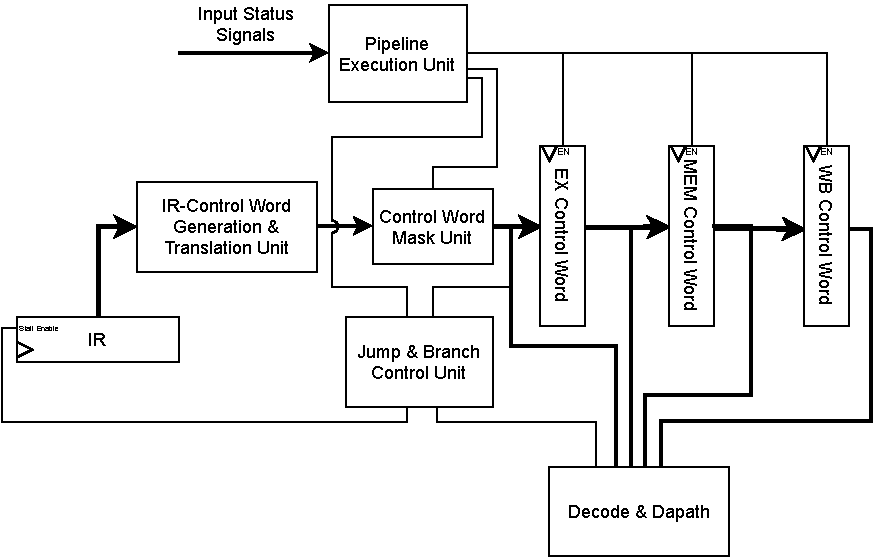
\includegraphics[width=0.72\textwidth]{chapters/2_dlx/images/DLX-Cu.pdf}
    \caption{Schematic of the DLX Control Unit}
    \label{dlx:cu:schematic}
\end{figure} 

It is made mainly by the following components:

\begin{itemize}
    \item IR-Control Word Generation \& Translation Unit: its role is to take the instruction given as input and output, a valid Control Word related to that instruction.
    \item Pipeline Execution Unit: it's in charge of controlling the Pipeline Flow and stop it in case of needs and/or masking the actual Control Word to prevent its propagation through the chain in case of Hazards.
    \item Control Word Mask Unit: when the \emph{Pipeline Execution Unit} signals to mask the control word, this unit will do it by disabling all the bits in the CW that referees to the stage enabling signals.
    \item Jump \& Branch Control unit: given the Control Word and other internal control signals, its job is to manage (by enabling or disabling them) signals like \emph{CALL}, \emph{RET}, \emph{JUMP\_EN} and \emph{IF\_STALL}.
\end{itemize}

% \begin{box_implementation_details}
%     {\large{\textbf{Implementation details: CW Generation Unit}}}
%   \newline
%     As said, the \emph{IR-Control Word Generation \& Translation Unit} is in charge of taking as input the actual instruction and to give as output a valid control word. How the mapping IR$\xrightarrow$CW is done?\\
% \end{box_implementation_details}


\section{Memory Interface}

The DLX processor has a Harvard architecture, with two 32-bit data buses carrying instructions and data respectively. Only load and store instructions can access data from Data Memory. The data are stored in memory in a Big-Endian format.\\

\begin{center}
    \begin{bytefield}[endianness=big,bitwidth=0.03\linewidth]{32}
    \bitheader{0, 7, 8, 15, 16, 23, 24, 31} \\
    \bitbox{32}{Word at address A}\\
    \bitbox{16}{Half at address A} & \bitbox{16}{Word at address A+2}\\
    \bitbox{8}{Byte at address A} & \bitbox{8}{Byte at address A+1} & \bitbox{8}{Byte at address A+2} & \bitbox{8}{Byte at address A+3}\\
    \end{bytefield}
\end{center}

The third RAM required, the one for the register file, is not under the User's direct access. It's managed as a Stack memory by the Register File for automatic subroutines management, and it has a dedicated interface. It can be merged with the Data Memory with external logic.\\

All the subsequent paragraphs are referred in the same way to all the three memory types.

\subsection{Signals and Timing}
The signals in the DLX processor bus interface can be grouped into tree categories:
\begin{itemize}
    \itemsep0sp
    \item Address class signals
    \item Memory Request signals
    \item Data class signals
\end{itemize}

The \emph{Address class signals} are:
\begin{itemize}
    \itemsep0sp
    \item A{[31:0]}
    \item DATA\_SIZE{[1:0]} \emph{or MAS{[1:0]}}
\end{itemize}

The \emph{Memory Request signals} are:
\begin{itemize}
    \itemsep0sp
    \item Enable
    \item $R\overline{W}$
    \item Ready
\end{itemize}

Moreover, all the memories connected must agree on a specific protocol both for writing and reading operations. The most important thing to take under consideration is the \emph{Ready} signal: it must be high only when the operation is completed. For example, after a data read, the \emph{Ready} stays at 1 only when the data is valid. If, meanwhile, the address changes, the \emph{Ready} signal must go off.

\begin{center}
    \begin{tikztimingtable}[%
        timing/dslope=0.2,
        timing/.style={x=8ex,y=2ex},
        x=8ex,
        timing/rowdist=3ex,
        timing/name/.style={font=\sffamily\scriptsize}
    ]
        \busref{CLK}                & 16{c} \\
        \busref[31:0]{Address}      & 2x 1D{$A_1$} 2D{$A_2$} 1X 1D{$A_4$} UX \\
        \busref[1:0]{MAS}           & 2x 1D{WORD 00} 2D{HALF 01} X 1D{BYTE 10} 2X\\
        \busref{Enable}             & 1L 2H HL HL L\\
        \busref{$RnW$}              & 1L 2H 2H LH L\\
        Ready                       & ll lh lh hh ll lh LL\\
        \busref[31:0]{Data In}      & 2x 2x 1X 1X 1X 1D{$D_1$} XX \\
        \busref[31:0]{DATA Out}      & 2x x1d{$D_1$} x3d{$D_2$} 4X  \\
        \extracode
        \begin{pgfonlayer}{background}
        \begin{scope}[semitransparent ,semithick]
        \vertlines[darkgray,dotted]{0.5,1.5 ,...,8.0}
        \end{scope}
        \end{pgfonlayer}
    \end{tikztimingtable}
\end{center}


If the Memory in use can't accomplish this timing, an external \emph{Memory Control Unit} must be placed between the CPU and the Memory.

\subsection{Memory Addressing}
A[31:0] is the 32-bit address bus that specifies the address for the transfer. All addresses are byte addresses, so a burst of word accesses results in the address bus incrementing by four for each cycle.\\

The address bus provides 4GB of linear addressing space, and this can be used externally in different manners, like in an SoC with memory-mapped peripherals that share the same address space.\\

When word access is signaled, the memory system ignores the bottom two bits, A[1:0], and when halfword access is signaled, the memory system ignores the bottom bit, A[0]. However, the core already masks the two LSBs when needed.

\subsection{Memory Data Size: the MAS[1:0] signal}
\label{mas}

The \emph{MAS[1:0]} bus encodes the size of the transfer. The DLX processor can transfer word, halfword, and byte quantities and the processor indicates the size of the transfer through this signal.\\

The \emph{MAS[1:0]} signal is supposed to be used in combination with \emph{A[1:0]} to know precisely which byte is taken under consideration during an operation.

\subsection{Memory Read}

When a half-word or byte read is performed, a 32-bit memory system can return the complete 32-bit word for simplicity, and the processor extracts the valid half-word or byte field from it as shown in Table \ref{table:memory_read_configuration}. Other byte lanes will be ignored. For 8 and 16 bit memories, the data must be placed on the right byte lanes in the data bus.

\begin{table}[H]
    \centering
    \begin{tabular}{|l|c|l|l|}
    \hline
        DATA\_SIZE[1:0] & A[1:0] & D[31:0] & DLX Register \\ \hline
        00 WORD & 00 & \texttt{0xAABBCCDD} & \texttt{0xAABBCCDD} \\ \hline
        01 HALF & 00 & \texttt{0xAABB----} & \texttt{0x0000AABB} \\ \hline
        01 HALF & 10 & \texttt{0x----CCDD} & \texttt{0x0000CCDD} \\ \hline
        10 BYTE & 00 & \texttt{0xAA------} & \texttt{0x000000AA} \\ \hline
        10 BYTE & 01 & \texttt{0x--BB----} & \texttt{0x000000BB} \\ \hline
        10 BYTE & 10 & \texttt{0x----CC--} & \texttt{0x000000CC} \\ \hline
        10 BYTE & 11 & \texttt{0x------DD} & \texttt{0x000000DD} \\ \hline
    \end{tabular}
    \caption{How data are read by the CPU in different MAS configurations}
    \label{table:memory_read_configuration}
\end{table}

\subsection{Memory Write}

Instead, when the DLX processor performs a byte or half-word write, the data being written is replicated across the data bus, as shown in Figure \ref{figure:dlx:memory_replication}. The memory system can use the most convenient copy of the data.

A writable memory system must be capable of performing a write to any single byte in the memory system. This is required for the correct working of the DLX. 

\begin{figure}[h]
    \centering
    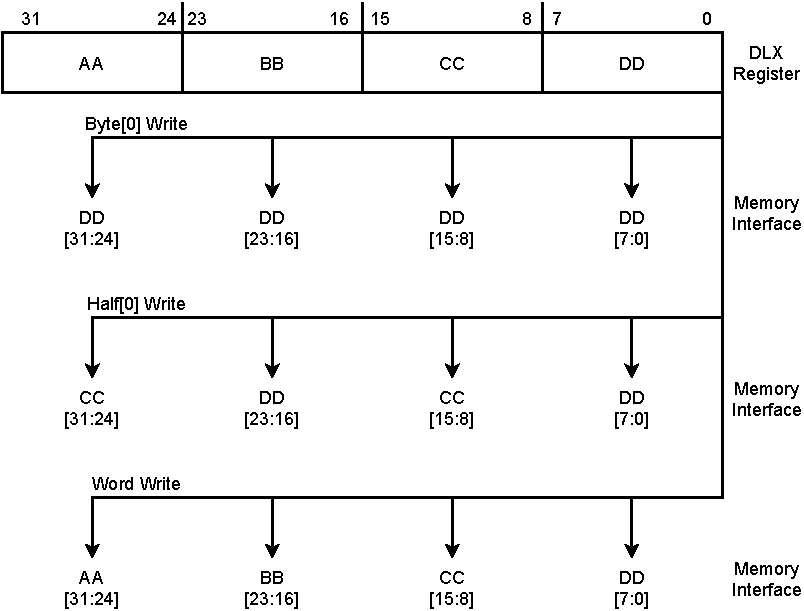
\includegraphics[width=.57\textwidth]{chapters/2_dlx/images/DLX-MemoryWordReplication.pdf}
    \caption{Data Write Replication}
    \label{figure:dlx:memory_replication}
\end{figure} 

\newpage
\section{Instruction Set}
\label{section:inst_set}

The Instruction Set supported by the DLX is made of different instructions, in particular regarding Integer operations. Instructions are on 32 bit and are grouped in 3 different types:\\

\begin{figure}[ht]
    \begin{center}
        \begin{bytefield}[endianness=big,bitwidth=0.03\linewidth]{32}
            \bitheader{0, 10, 11, 15, 16, 20, 21, 25, 26, 31} \\
            \bitbox{6}{OP CODE} & \bitbox{5}{REG SRC1} & \bitbox{5}{REG SRC2} &  \bitbox{5}{REG DEST} & \bitbox{11}{FUNC CODE} \\
        \end{bytefield}
    \end{center}
    \caption{R-Type}
    \label{fig:rtype}
\end{figure}

\begin{figure}[ht]
    \begin{center}
        \begin{bytefield}[endianness=big,bitwidth=0.03\linewidth]{32}
            \bitheader{0, 15, 16, 20, 21, 25, 26, 31} \\
            \bitbox{6}{OP CODE} & \bitbox{5}{REG SRC} & \bitbox{5}{REG DEST} &  \bitbox{16}{IMMEDIATE} \\
        \end{bytefield}
    \end{center}
    \caption{I-Type}
    \label{fig:itype}
\end{figure}

\begin{figure}[ht]
    \begin{center}
        \begin{bytefield}[endianness=big,bitwidth=0.03\linewidth]{32}
            \bitheader{0, 25, 26, 31} \\
            \bitbox{6}{OP CODE} & \bitbox{26}{IMMEDIATE} \\
        \end{bytefield}
    \end{center}
    \caption{J-Type}
    \label{fig:jtype}
\end{figure}

In particular, all of them have in common the \emph{OP CODE} field, used to identify the instruction.

\subsection{R-Type Instructions}

R-Type Instructions are called in this way because they operates only between registers. They all have in common the \emph{OP CODE} equal to \texttt{0b00000} and each instruction is differentiated from another one thanks to the \emph{FUNC CODE} field, as shown in Table \ref{table:r_type} and Table \ref{table:r_type_test}.

\begin{table}[H]
\begin{tabularx}{\textwidth}{|l|c|l|l|X|}
    \hline
    MNEMONIC & FUNC CODE & EXAMPLE & OPERATION & DESCRIPTION \\ 
    \hline
    SLL & \texttt{0x04} & \texttt{SLL R3, R2, R1} & $R3 \leftarrow R2 \ll R1$ & Logical shift left\\ 
    \hline
    SRL & \texttt{0x06} & \texttt{SRL R3, R2, R1} & $R3 \leftarrow R2 \gg R1$ & Logical shift right\\ 
    \hline
    SRA & \texttt{0x07} & \texttt{SRA R3, R2, R1} & $R3 \leftarrow R2 \gg R1$ & Arithmetic shift right\\ 
    \hline
    ROR & \texttt{0x08} & \texttt{ROR R3, R2, R1} & $R3 \leftarrow R2 \circlearrowright R1$ & Right rotation\\ 
    \hline
    ROL & \texttt{0x09} & \texttt{ROL R3, R2, R1} & $R3 \leftarrow R2 \circlearrowleft R1$ & Left rotation\\ 
    \hline
    MUL & \texttt{0x0E} & \texttt{MUL R3, R2, R1} & $R3 \leftarrow R2 * R1$ & Integer multiplication\\ 
    \hline
    ADD & \texttt{0x20} & \texttt{ADD R3, R2, R1} & $R3 \leftarrow R2 + R1$ & Integer Add\\ 
    \hline
    ADDU & \texttt{0x21} & \texttt{ADDU R3, R2, R1} & $R3 \leftarrow R2 + R1$ & Integer Add\\ 
    \hline
    SUB & \texttt{0x22} & \texttt{SUB R3, R2, R1} & $R3 \leftarrow R2 - R1$ & Integer subtraction\\ 
    \hline
    SUBU & \texttt{0x23} & \texttt{SUBU R3, R2, R1} & $R3 \leftarrow R2 - R1$ & Integer subtraction\\ 
    \hline
    AND & \texttt{0x24} & \texttt{AND R3, R2, R1} & $R3 \leftarrow R2 \texttt{\&} R1$ & Bitwise AND\\ 
    \hline
    OR & \texttt{0x25} & \texttt{OR R3, R2, R1} & $R3 \leftarrow R2 \mid R1$ & Bitwise OR\\ 
    \hline
    XOR & \texttt{0x26} & \texttt{XOR R3, R2, R1} & $R3 \leftarrow R2 \oplus R1$ & Bitwise XOR\\ 
    \hline
\end{tabularx}
\caption{R-TYPE Instructions: logical and arithmetic}
\label{table:r_type}
\end{table}

\begin{table}[H]
\begin{tabularx}{\textwidth}{|l|c|l|l|X|}
    \hline
    MNEMONIC & FUNC CODE & EXAMPLE & OPERATION & DESCRIPTION \\ 
    \hline
    SEQ & \texttt{0x28} & \texttt{SEQ R3, R2, R1} & $R3 \leftarrow R2 == R1$ & 1 if R2 equal R1\\ 
    \hline
    SNE & \texttt{0x29} & \texttt{SNE R3, R2, R1} & $R3 \leftarrow R2 != R1$ & 1 if R2 not equal R1\\ 
    \hline
    SLT & \texttt{0x30} & \texttt{SLT R3, R2, R1} & $R3 \leftarrow R2 < R1$ & 1 if R2 less R1\\ 
    \hline
    SGT & \texttt{0x31} & \texttt{SGT R3, R2, R1} & $R3 \leftarrow R2 > R1$ & 1 if R2 great R1\\ 
    \hline
    SLE & \texttt{0x32} & \texttt{SLE R3, R2, R1} & $R3 \leftarrow R2 \leq R1$ & 1 if R2 less or equal R1\\ 
    \hline
    SGE & \texttt{0x33} & \texttt{SGE R3, R2, R1} & $R3 \leftarrow R2 \geq R1$ & 1 if R2 great or equal R1\\ 
    \hline
    SLTU & \texttt{0x3A} & \texttt{SLTU R3, R2, R1} & $R3 \leftarrow R2 < R1$ & 1 if R2 unsigned less R1\\ 
    \hline
    SGTU & \texttt{0x3B} & \texttt{SGTU R3, R2, R1} & $R3 \leftarrow R2 > R1$ & 1 if R2 uns great R1\\ 
    \hline
    SLEU & \texttt{0x3C} & \texttt{SLEU R3, R2, R1} & $R3 \leftarrow R2 \leq R1$ & 1 if R2 uns less/eq R1\\ 
    \hline
    SGEU & \texttt{0x3D} & \texttt{SGEU R3, R2, R1} & $R3 \leftarrow R2 \geq R1$ & 1 if R2 uns great/eq R1\\ 
    \hline
\end{tabularx}
\caption{R-TYPE Instructions: test instructions}
\label{table:r_type_test}
\end{table}

\subsection{Pseudo R-Type Instructions}

Here we find R-Type like operations: they work only with registers but have their OPCODE.

\begin{table}[H]
\begin{tabularx}{\textwidth}{|l|c|l|l|X|}
    \hline
    MNEMONIC & OP CODE & EXAMPLE & OPERATION & DESCRIPTION \\ 
    \hline
    JR & \texttt{0x12} & \texttt{JR R1} & $PC \leftarrow PC + R1$ & PC += R31\\ 
    \hline
    JALR & \texttt{0x13} & \texttt{JALR R1} & $R31 \leftarrow PC $ & R31 = actual PC\\ 
    & & & $PC \leftarrow PC + R1$ & PC += R1\\ 
    \hline
    RET & \texttt{0x1F} & \texttt{RET} & $PC \leftarrow R31$ & PC = R31\\ 
    & & & & Context Switch begins\\ 
    \hline
    NOP & \texttt{0x15} & \texttt{NOP} & & Does exactly nothing\\ 
    \hline
    TICKTMR & \texttt{0x34} & \texttt{TICKTMR R16} &  $R16 \leftarrow TICK TIMER $ & Get Tick Timer value\\ 
    \hline
\end{tabularx}
\caption{Pseudo R-TYPE Instructions: branch, jump and mix}
\label{table:r_type_jump}
\end{table}

\subsection{J-Type Instructions}

J-Type Instructions are groups of instructions made for code jump. Thanks to the structure of these instructions, long jumps can be executed (i.e. the relative address can be very big).

\begin{table}[H]
\begin{tabularx}{\textwidth}{|l|c|l|l|X|}
    \hline
    MNEMONIC & OP CODE & EXAMPLE & OPERATION & DESCRIPTION \\ 
    \hline
    J & \texttt{0x02} & \texttt{J LABEL} & $PC \leftarrow PC + LABEL$ & PC += rel label\\ 
    \hline
    JAL & \texttt{0x03} & \texttt{JAL LABEL} & $R31 \leftarrow PC $ & R31 = actual PC\\ 
    & & & $PC \leftarrow PC + LABEL$ & PC += rel label\\ 
    \hline
    CALL & \texttt{0x1E} & \texttt{CALL LABEL} & $R31 \leftarrow PC $ & R31 = actual PC\\ 
    & & & $PC \leftarrow PC + LABEL$ & PC += rel label\\ 
    & & & & Context Switch begins\\ 
    \hline
\end{tabularx}
\caption{J-TYPE Instructions}
\label{table:j_type}
\end{table}

\newpage
\subsection{I-Type Instructions}

I-Type instructions support immediate operands, as shown in Table \ref{table:i_type_airth_logic}. 

\begin{table}[H]
\begin{tabularx}{\textwidth}{|l|c|l|l|X|}
    \hline
    MNEMONIC & OP CODE & EXAMPLE & OPERATION & DESCRIPTION \\ 
    \hline
    ADDI & \texttt{0x08} & \texttt{ADDI R3, R0, \#2} & $R3 \leftarrow R0 + 2$ & Integer Add\\ 
    \hline
    ADDUI & \texttt{0x09} & \texttt{ADDUI R3, R2, \#2} & $R3 \leftarrow R2 + 2$ & Integer Add\\ 
    \hline
    SUBI & \texttt{0x0A} & \texttt{SUBI R3, R2, R1} & $R3 \leftarrow R2 - R1$ & Integer subtraction\\ 
    \hline
    SUBUI & \texttt{0x0B} & \texttt{SUBUI R3, R2, R1} & $R3 \leftarrow R2 - R1$ & Integer subtraction\\ 
    \hline
    ANDI & \texttt{0x0C} & \texttt{ANDI R3, R2, R1} & $R3 \leftarrow R2 \texttt{\&} R1$ & Bitwise AND\\ 
    \hline
    ORI & \texttt{0x0D} & \texttt{ORI R3, R2, R1} & $R3 \leftarrow R2 \mid R1$ & Bitwise OR\\ 
    \hline
    XORI & \texttt{0x0E} & \texttt{XORI R3, R2, R1} & $R3 \leftarrow R2 \oplus R1$ & Bitwise XOR\\ 
    \hline
    LHI & \texttt{0x0F} & \texttt{LHI R3, \#0xABCD} & $R3 \leftarrow \texttt{0xABCD0000}$ & Load Upper Half\\ 
    \hline
    SLLI & \texttt{0x14} & \texttt{SLLI R3, R2, \#1} & $R3 \leftarrow R2 \ll 1$ & Logical shift left\\ 
    \hline
    SRLI & \texttt{0x16} & \texttt{SRLI R3, R2, \#1} & $R3 \leftarrow R2 \gg 1$ & Logical shift right\\ 
    \hline
    SRAI & \texttt{0x17} & \texttt{SRAI R3, R2, \#1} & $R3 \leftarrow R2 \gg 1$ & Arithmetic shift right\\ 
    \hline
\end{tabularx}
\caption{I-TYPE Instructions: logical and arithmetic}
\label{table:i_type_airth_logic}
\end{table}


\begin{table}[H]
\begin{tabularx}{\textwidth}{|l|c|l|l|X|}
    \hline
    MNEMONIC & OP CODE & EXAMPLE & OPERATION & DESCRIPTION \\ 
    \hline
    SEQI & \texttt{0x18} & \texttt{SEQI R3, R2, \#1} & $R3 \leftarrow R2 == 1$ & 1 if R2 equal 1\\ 
    \hline
    SNEI & \texttt{0x19} & \texttt{SNEI R3, R2, \#1} & $R3 \leftarrow R2 != 1$ & 1 if R2 not equal 1\\ 
    \hline
    SLTI & \texttt{0x1A} & \texttt{SLTI R3, R2, \#1} & $R3 \leftarrow R2 < 1$ & 1 if R2 less 1\\ 
    \hline
    SGTI & \texttt{0x1B} & \texttt{SGTI R3, R2, \#1} & $R3 \leftarrow R2 > 1$ & 1 if R2 great 1\\ 
    \hline
    SLEI & \texttt{0x1C} & \texttt{SLEI R3, R2, \#1} & $R3 \leftarrow R2 \leq 1$ & 1 if R2 less or equal 1\\ 
    \hline
    SGEI & \texttt{0x1D} & \texttt{SGEI R3, R2, \#1} & $R3 \leftarrow R2 \geq 1$ & 1 if R2 great or equal 1\\ 
    \hline
    SLTUI & \texttt{0x3A} & \texttt{SLTUI R3, R2, \#1} & $R3 \leftarrow R2 < 1$ & 1 if R2 unsigned less 1\\ 
    \hline
    SGTUI & \texttt{0x3B} & \texttt{SGTUI R3, R2, \#1} & $R3 \leftarrow R2 > 1$ & 1 if R2 uns great 1\\ 
    \hline
    SLEUI & \texttt{0x3C} & \texttt{SLEUI R3, R2, \#1} & $R3 \leftarrow R2 \leq 1$ & 1 if R2 uns less/eq 1\\ 
    \hline
    SGEUI & \texttt{0x3D} & \texttt{SGEUI R3, R2, \#1} & $R3 \leftarrow R2 \geq 1$ & 1 if R2 uns great/eq 1\\ 
    \hline
\end{tabularx}
\caption{I-TYPE Instructions: test instructions}
\label{table:i_type_test}
\end{table}


\begin{table}[H]
\begin{tabularx}{\textwidth}{|l|c|l|l|X|}
    \hline
    MNEMONIC & OP CODE & EXAMPLE & OPERATION & DESCRIPTION \\ 
    \hline
    LB & \texttt{0x20} & \texttt{LB R1, 40(R2)} & $R1 \leftarrow MEM[ R2 + 40 ] $ & Load Byte / Sign Ext\\ 
    \hline
    LH & \texttt{0x21} & \texttt{LH R1, 40(R2)} & $R1 \leftarrow MEM[ R2 + 40 ] $ & Load Half / Sign Ext\\ 
    \hline
    LW & \texttt{0x23} & \texttt{LW R1, 40(R2)} & $R1 \leftarrow MEM[ R2 + 40 ] $ & Load Word / Sign Ext\\ 
    \hline
    LBU & \texttt{0x24} & \texttt{LBU R1, 40(R2)} & $R1 \leftarrow MEM[ R2 + 40 ] $ & Load Byte\\ 
    \hline
    LHU & \texttt{0x25} & \texttt{LHU R1, 40(R2)} & $R1 \leftarrow MEM[ R2 + 40 ] $ & Load Half\\ 
    \hline
    SB & \texttt{0x28} & \texttt{SB 40(R2), R1} & $MEM[ R2 + 40 ] \leftarrow R1 $ & Store Byte \\ 
    \hline
    SH & \texttt{0x29} & \texttt{SH 40(R2), R1} & $MEM[ R2 + 40 ] \leftarrow R1 $ & Store Half \\ 
    \hline
    SW & \texttt{0x2B} & \texttt{SW 40(R2), R1} & $MEM[ R2 + 40 ] \leftarrow R1 $ & Store Word \\ 
    \hline
\end{tabularx}
\caption{I-TYPE Instructions: Load \& Store}
\label{table:i_type_loadstore}
\end{table}

\begin{table}[H]
\begin{tabularx}{\textwidth}{|l|c|l|l|X|}
    \hline
    MNEMONIC & OP CODE & EXAMPLE & OPERATION & DESCRIPTION \\ 
    \hline
    BEQZ & \texttt{0x04} & \texttt{BEQZ R1, LABEL} & $PC \leftarrow PC + LABEL$ & $R1 = 0$ ?\\ 
    & & & & PC += label\\
    \hline
    BNEZ & \texttt{0x05} & \texttt{BNEZ R1, LABEL} & $PC \leftarrow PC + LABEL$ & $R1 \neq 0$ ?\\ 
    & & & & PC += label\\
    \hline
    BGT & \texttt{0x30} & \texttt{BGT R1, R2, LABEL} & $PC \leftarrow PC + LABEL$ & $R1 > R2$ ?\\ 
    & & & & PC += label\\
    \hline
    BGE & \texttt{0x31} & \texttt{BGE R1, R2, LABEL} & $PC \leftarrow PC + LABEL$ & $R1 \ge R2$ ?\\ 
    & & & & PC += label\\
    \hline
    BLT & \texttt{0x32} & \texttt{BLT R1, R2, LABEL} & $PC \leftarrow PC + LABEL$ & $R1 < R2$ ?\\ 
    & & & & PC += label\\
    \hline
    BLE & \texttt{0x33} & \texttt{BLE R1, R2, LABEL} & $PC \leftarrow PC + LABEL$ & $R1 \le R2$ ?\\ 
    & & & & PC += label\\
    \hline
\end{tabularx}
\caption{I-TYPE Instructions: Conditional Branch Instructions}
\label{table:i_type_branch}
\end{table}